% Chapter Template

\chapter{Diseño e implementación} % Main chapter title

\label{Chapter2} % for referencing this chapter elsewhere, use \ref{ChapterX}

En esta sección explicaremos detenidamente los distintos pasos que se llevaron a cabo para obtener la aplicación final. \\

Como se ha indicado en la introducción, la tarea fundamental de nuestra aplicación consiste en procesar lo que diga el usuario para poder comparar su pronunciación con la de un nativo. La aplicación está enfocada al tratamiento y comparación del sonido y puede ser incluida por cualquier otra aplicación con interfaz de usuario, ya sea una aplicación móvil, de escritorio u online. Teniendo esto en cuenta se diseñó la aplicación.\\

Una de las decisiones fue programar en lenguaje Java ya que es con el que tengo más dominio y experiencia. \todo{REVISAR porque tiene que tener sentido con que al principio era android } % REVISAR
Además, Java tiene muchas bibliotecas y recursos que hemos tratado de aprovechar. El código puede encontrarse REF \cite{REF} % REF
 y es código abierto y libre. La estructura del código de la aplicación se puede encontrar en esta memoria. REF \cite{REF} \\ % REF

Daremos en primer lugar una visión general de todo el programa. Cuando una persona use el programa se grabará diciendo una frase indicada y la aplicación dirá si la pronunciación ha sido suficientemente buena y leal a la de un nativo. Por ello, el primer paso es obtener un audio directamente del micrófono del medio que esté usando el usuario. El sonido capturado se guardará digitalmente como una secuencia de intensidades que contienen toda la información de audio, este contiene muchas frecuencias no útiles para nuestro objetivo de comparar voces pronunciando la misma frase. Por ello habrá una etapa de filtrado. Después se hará una transformación de Fourier a la señal dividida en segmentos, que nos dará el valor de los impulsos por frecuencia de los segmentos. Aprovecharemos que se encuentra en el dominio de la frecuencia para quitar el sonido de fondo. Y con el espectrograma resultante de la transformación limpia nos quedaremos con la matriz bidimensional asociada, donde cada valor representa la intensidad del impulso por tiempo (segmento) y frecuencia. Esta matriz se puede interpretar como una imagen donde el color en cada punto se consigue a partir del elemento correspondiente en la matriz. Una vez que tenemos la imagen, se hace una detección de blobs o regiones para distinguir las zonas más destacables o sobresalientes de la imagen. Con esto conseguiremos una matriz de valores con más contraste y lista para ser comparada con otra matriz de la misma clase, teniendo en cuenta que las dimensiones de las matrices pueden variar ya sea por la velocidad o volumen del hablante.\\

En el resto de la sección daremos los detalles de estos pasos, dando en primer lugar una explicación teórica y desarrollando después los principales aspectos de implementación.

%----------------------------------------------------------------------------------------
%	SECTION 1
%----------------------------------------------------------------------------------------

\section{Capturando la voz}

Cuando el usuario grabe su voz para ser procesada debemos capturar el audio en un formato que nos facilite su tratamiento. Grabar en formato de audio \emph{raw} nos da total control y visualización de los datos capturados.
Cuando emitimos el sonido para ser grabado emitimos una señal analógica (continua) que el micrófono captura y guarda en forma de señal digital (discreta). 
La transformación de esta señal analógica a digital se hace a través de un proceso llamado muestreo.
En procesamiento de señales, el muestreo es la reducción de una señal continua a una señal discreta. Consiste en tomar muestras de una señal analógica a una frecuencia o tasa de muestreo (\emph{sample rate}) constante, para cuantificarlas y codificarlas posteriormente. La cuantificación consiste en atribuir un valor finito (discreto) de amplitud a cada muestra, un valor dentro de un conjunto específico de valores que luego es codificado en bits.\\

En la figura \ref{fig:sampling} podemos observar cómo se toman muestras discretas $S_i$ de la señal continua $S(t)$ cada $T$ unidades de tiempo.

\begin{figure}[th]
\centering
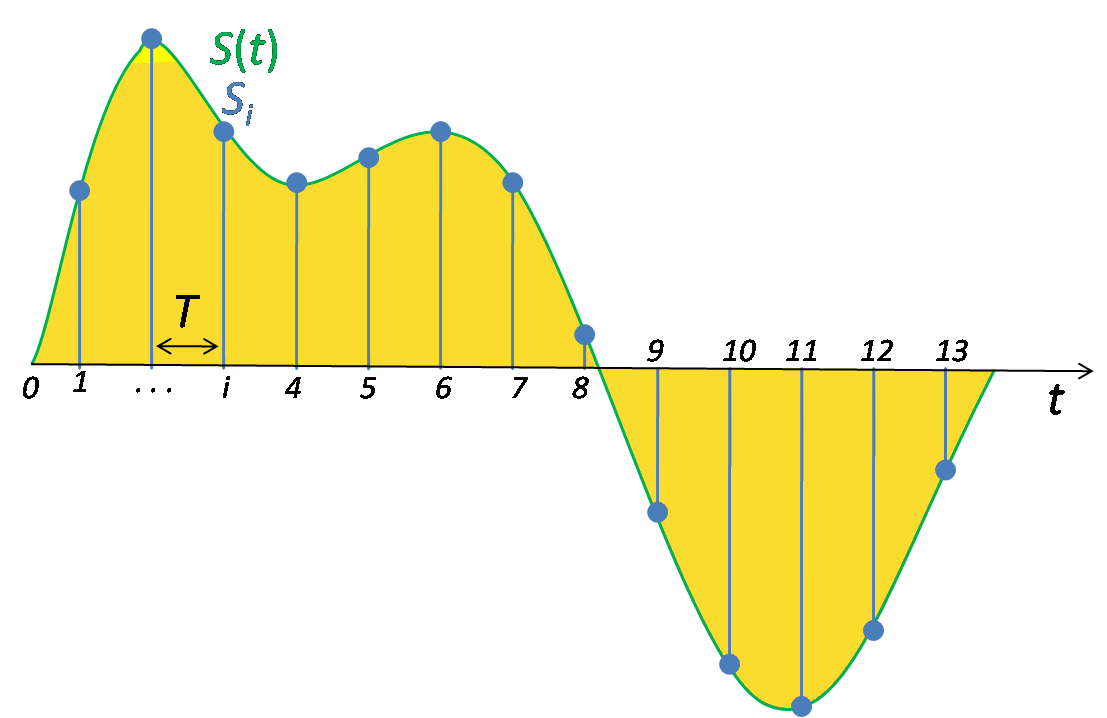
\includegraphics[width=7cm]{Figures/Signal_Sampling}
\decoRule
\caption[Muestreo]{Muestreo de una señal continua para obtener una señal discreta.}
\label{fig:sampling}
\end{figure}

Por tanto, el sonido se graba en muestras discretas y la velocidad con la que se toman estas muestras se llama \emph{sample rate} o frecuencia de muestreo. \\

El método más común de representar sonido analógico digitalmente modulación por impulsos codificados (PCM por sus siglas en inglés \emph{Pulse-code modulation}\cite{REF}). \todo{Falta referencia}{}% REF de pcm
PCM es un procedimiento de modulación que transforma una señal analógica en una secuencia de bits. Además, es la forma estándar de audio digital en ordenadores, discos compactos, telefonía digital y otras aplicaciones similares. \cite{REF}% REF
 
 En un flujo PCM la intensidad de una señal analógica es muestreada regularmente en intervalos uniformes, y cada muestra es cuantizada al valor más cercano dentro de un rango de pasos digitales. \\

Para determinar cómo será la señal digital y medir su fidelidad a la señal analógica, el flujo PCM tiene dos propiedades básicas:
\begin{itemize}
\item Frecuencia de muestreo: el número de veces por segundo que se toma una muestra
\item \emph{Bit depth}: el número de posibles valores digitales usados para representar cada muestra. 
\end{itemize}

¿Qué valores le daremos a estas variables?

En cuanto a la frecuencia de muestreo, hay que tener en cuenta los límites de audición o rango de frecuencias que un humano percibe, que se encuentran entre los 20 y 20K Hz. Por esto, en música y grabaciones en general se muestrea a 44.1 kHz, es decir, se toman 44.1 mil muestras de la señal analógica por segundo.

Por otro lado, las señales de voz o \emph{speech}, que solo contienen la voz humana, se suelen tomar menos muestras por segundo. La mayoría de fonemas se encuentra entre 100 y 4K Hz, permitiendo un \emph{sample rate} de 8 kHz.  \cite{REF}.% REF

Usaremos un ratio de 44.1 kHz por ser más común y bastante utilizado. Pero tendremos en cuenta más adelante el rango de frecuencias en que se mueve la señal de la voz. \\

\begin{figure}[th]
\centering
\includegraphics[width=7cm]{Figures/LimAudicion}
\decoRule
\caption[LimAudicion]{Límites de audición humanos.}
\label{fig:limAudicion}
\end{figure}

Para explicar por qué se escoge como frecuencia el doble del máximo valor del rango usaremos el teorema de muestreo de Nyquist-Shannon, que dice que al tomar muestras de una señal con una frecuencia que sea el doble de la frecuencia máxima de la señal, dichas muestras contendrán toda la información necesaria para reconstruir la señal original. Es decir, se podrá reconstruir la señal analógica a partir de la digital. Y por eso siempre se toma ese criterio para elegir la frecuencia de muestreo.\\

Y en cuanto al \emph{bit depth}, es decir, el número de bits de información para cada muestra que se corresponde directamente con el valor cuantificado de la muestra, elegiremos uno común. Los \emph{bit depth} más comunes para PCM son 8, 16, 20 o 24 bits por muestra. Nosotros usaremos un \emph{short} con signo que son 16 bits. Un \emph{bit depth} de 16-bit nos dará 65536 niveles. \\

Otra variable que debemos configurar cuando grabamos audio es el número de canales, en este caso un solo canal o monocanal será suficiente, no necesitamos más. Un canal de audio es un canal o pista donde los elementos grabados tienen su propio área en la grabación, cuando escuchamos una grabación con varios canales, todos ellos suenan simultáneamente. Cuando se almacena música se usan dos canales (estéreo) y más de dos en el caso de películas para conseguir un mejor efecto.\\

En cuanto al formato del archivo de audio que obtenemos, como hemos dicho, intentaremos que sea formato \emph{raw} o PCM, es decir, una secuencia de palabras de 16 bits que representan la intensidad de cada muestra tomada de la señal. \\

En cuanto a la implementación, dos de los formatos contenedores de audio más conocidos, WAV y AIFF, utilizan el formato PCM. Nosotros utilizaremos WAVE (\emph{Waveform Audio File Format}) conocido como WAV, que es en pocas palabras, un \emph{raw} con cabecera donde se tiene el tamaño del archivo, el tamaño de la cabecera, el formato de audio (PCM), la frecuencia de muestreo, número de canales (1 o 2 ya que WAV es solo para audio digital), el número de bits por muestra y otros campos como se muestra en la imagen \ref{fig:waveFormat}. Quitar esa cabecera y obtener los datos en crudo es muy simple: tan solo debemos descartar los primeros 44 bits y guardamos el resultado en un \file{.raw}. Nos quedamos con lo que llama \code{data} que es el audio en bruto y se encuentra codificado con sistema \emph{little-endian}, esto quiere decir que el byte más significativo de los dos que forman las palabras de 16 bits es el segundo y, por tanto, se almacena en primer lugar.

\begin{figure}[th]
\centering
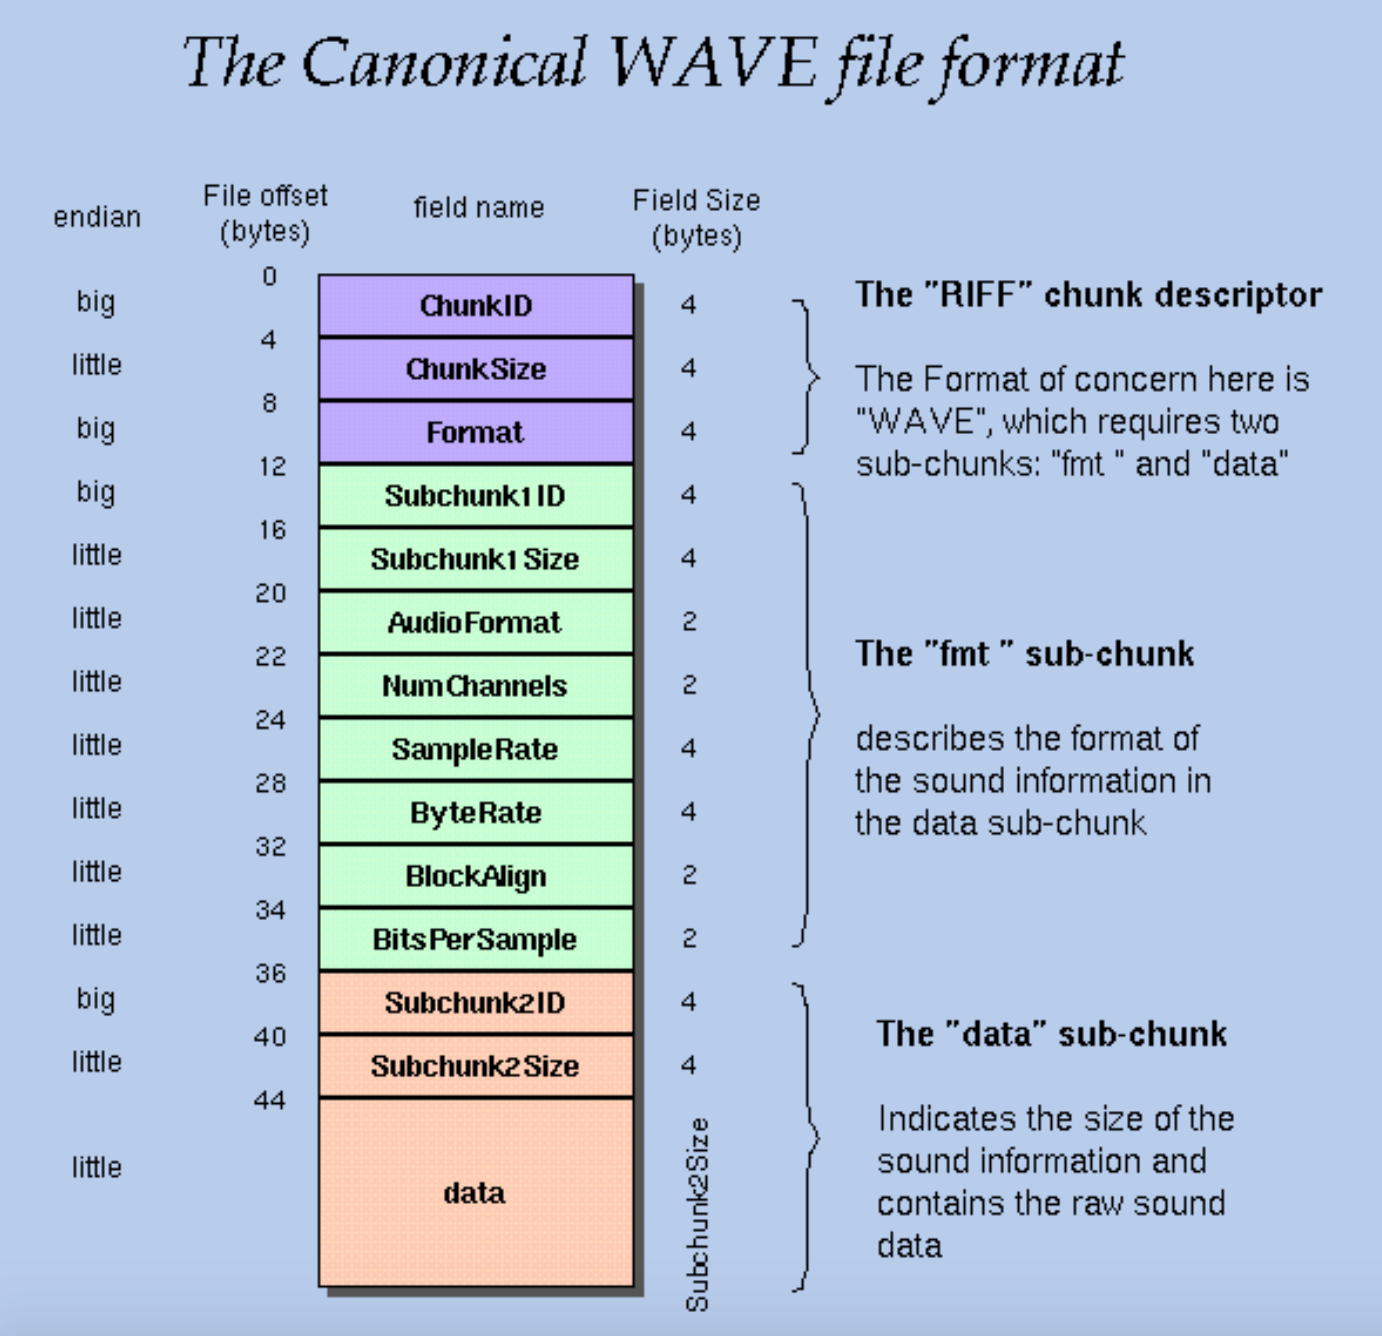
\includegraphics[width=7cm]{Figures/wave_format}
\decoRule
\caption[waveFormat]{Formato de archivos WAVE}
\label{fig:waveFormat}
\end{figure}

En resumen los ajustes que usaremos para capturar audio en formato WAV serán los siguientes:
\begin{itemize}
\item Codificación 16-bit PCM. 
\item Un solo canal o monocanal.
\item Frecuencia de muestreo: 44.1 kHz
\item Sistema \emph{little-endian} para almacenar los bytes.
\end{itemize}

En nuestro caso, hemos llevado a cabo esta captura de voz con la aplicación de captura y edición de audio Audacity \cite{REF} %REF a Audacity
, que es software libre y multiplataforma. En Audacity puedes especificar las configuraciones que indicamos en la descripción teórica que hemos presentado anteriormente; al leer un fichero raw será necesario indicar estos ajustes.

La forma de obtener el archivo de audio wav o raw es abierta. Usar Audacity es lo que nosotros hemos hecho pero se pueden obtener de muchas otras formas. Por ejemplo, un dato interesante es que todo dispositivo Android soporta la captura de audio con 1 canal a 44.1 kHz en codificación 16-bit PCM.\\

Ya tenemos hecho el primer paso, hemos conseguido los datos de audio en un formato que podemos manipular. El audio grabado está en bruto, lo siguiente será quitarle el ruido y frecuencias no útiles.

%-----------------------------------
%	SUBSECTION 1
%-----------------------------------
\subsection{Subsection 1}

Nunc posuere quam at l



